\documentclass[main.tex]{subfiles}
% IMPLEMENTATION
\begin{document}
  
  In this chapter I hope to give a conceptual overview of the technological state of the software. For details please consult the \textit{javadoc}.
  
  \section{Data Format}
    \label{sec:impl:data}
    
    In order to correctly process data sets a family of dedicated \textit{java.util.Collection} implementations has been designed. Any \textit{DataSet} class holds a list of elements ordered by their position on an independent variable axis. This allows storing for example data points of a function $f(x)$ while allowing efficient access to the value mapping to $x=5$, without the need to search the list of data points directly.
    
    \begin{SCfigure}[][h]
      \centering
      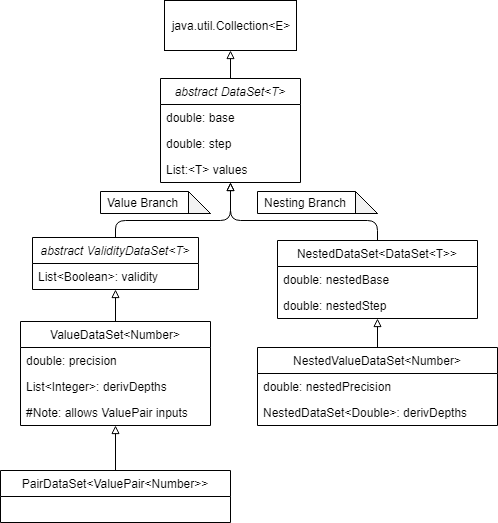
\includegraphics[width=0.55\linewidth]{figures/dataSetFamily}
      \captionsetup{format=plain, indention=1.0cm}
      \caption{The DataSet family used to store information on lists of data points. The family is split between the Value Branch (left) and the Nested Branch (right). The former is used to directly store one dimensional lists of data points, while the latter is used to store other DataSet objects and hence allow theoretically infinite dimensions. \\
      Only the fields that each class contains are shown, with functionality based on these and the classes' objectives omitted. See \Cref{cha:maint} for further details. \\
      Note that one dimensional means that there is one independent variable.}
      \label{fig:dataSetFam}
    \end{SCfigure}
    
    \subsection{Versatility}
    
      The DataSet classes were kept as versatile as possible such that future development should not be impeded by design decisions at this point. 
      \\\\
      They extend \textit{java.util.Collection} in order to take advantage of its iterator qualities, enforce well established architectural patterns and help clarify its design and use. However, implementing the \textit{java.uti.List} interface, while at first glance appearing more sensible due to the ordered nature of \textit{DataSet} entries, would create conflicts between the intended use of  \textit{DataSet} and the specified characteristics of a \textit{List}.
      \\\\
      Unless required by the set's functionality, any class can be stored in it, in order to minimise unnecessary constraints. This is in spite of the fact that for most if not all applications the \textit{Double} class will likely be the most advantageous. For example, while currently there is no reason to make use of GPU processing, this would likely require the use of \textit{Float} instead. Also, non-numerical classes are currently allowed in those classes that do not specifically deal with numerical entries. This is for the most part to allow the nesting of \textit{DataSet} objects, but theoretically offers much more functionality.
    
    \subsection{Principle}
      \label{sec:impl:dataPrinciple}
      
      The core functionality of \textit{DataSet} classes is the ordering of their entries by their independent variable. Usually this variable is denoted $x$ or here \textit{xValue}. Entries can be assigned to a particular \textit{xValue}, potentially overriding the existing entry. More importantly, they can be retrieved by their \textit{xValue} efficiently. 
      \\\\
      \textit{DataSet} does this very simply by mapping between the \textit{index} of an entry and its \textit{xValue}. Internally entries are stored in an \textit{ArrayList}, with their \textit{xValue} defined as $xValue= base + index * step$. The \textit{DataSet} is assigned immutable $base$ and $step$ values such that all entries follow the same pattern. As such they can be retrieved by their \textit{xValue} by mapping back to their index. \Cref{fig:dataSetGraph} shows an example where the data points can be easily stored in this way. In essence data points are expected to be a distance of $step$ apart, starting with the first value at $xValue=base$. If the data points are not exactly a constant distance apart, but only approximately, a \textit{ValuePair} can be used as an entry, that stores both the \textit{yValue} and \textit{xValue}. The \textit{PairDataSet} is intended to facilitate this use.
      \\\\
      This principle can be extended to not only store one dimentional data points, but to store entire \textit{DataSet} objects in this manner. As stated previously, this allows the modelling of multi dimensional data. While this \textit{NestedDataSet} use is not very far developed at this time, it is intended to both allow storing and retrieving data in this fashion, as but most importantly to process it efficiently. Of particular interest will be to implement an iteration functionality that is capable of iterating and processing entries across different \textit{ValueDataSets} that are nested within a \textit{NestedValueDataSet}.
      
      \begin{figure}[h]
        \centering
        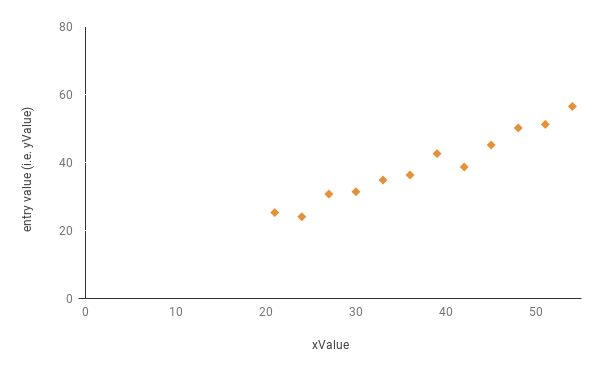
\includegraphics[width=0.75\linewidth]{figures/dataSetGraph}
        \caption{A conceptual example of a set of data points that can be stored in a \textit{DataSet}. In this example it would be initialised with $base=21$ and $step=3$, while the $precision$ should be chosen to reflect the presence of noise.}
        \label{fig:dataSetGraph}
      \end{figure}
      
      
  \section{Architecture}
    
    Given the limitations of the project to the foundation of the larger project, the only real product is what I dubbed the "Base" Module. This is a module that is intended to somewhat mirror the \textit{java.base} module architecturally, in the sense that it should be available throughout the larger project. Two other modules were prepared for demonstration purposes, the "generator" and a presentation  GUI.
    
    \subsection{Base Module}
      
      This module provides the data types that are described in \Cref{sec:impl:data} and should be used throughout the upcoming project for this reason alone. 
      \\\\
      In addition a number of "helper" classes are contained in this module. At this time these in particular provide the classification functionality discussed, as well as some other useful methods like a test whether two values should be considered equal within a given precision. This functionality is provided static, much like the java.util.Math functionality, for example.
      \\\\
      As the analysis becomes more and more complex it will quite definitely grow into a stand-alone module, though the currently existing classification is likely to remain as is. This is because it is comparatively light weight and provides information to enhance the usefulness of a DataSet. Further analysis would interpret the DataSet to a degree that all useful information is contained in the interpretation, and access to the original DataSet is no longer necessary.
      
    \subsection{Generator Module}
      
      The generator produces synthetic data on demand, that can be used to test as well as demonstrate the core functionality. It is entirely possible that this will remain useful in the future for exactly these reasons. However, due to its presentation only application so far only minimal quality assurance was enforced, with only superficial unit testing.
      \\\\
      The module makes use of some pseudo randomness, though scaffolding is present to allow reseeding and hence improving the randomness. Any of the classifiable functions can be generated, with adjustable noise and an arbitrary number of biases optional. The parameters that define the shape of the specified functions are defined by the aforementioned randomness, as well as the order in which functions are generated.
      \\\\
      For presentation purposes the module also contains a an adapter for the presentation GUI that could be reused.
      
    \subsection{GUI}
      
      The current GUI is only intended to allow university presentations and will be archived after this project. For the larger Oil and Gas project a GUI has been developed by another developer in JavaScript, but not well adapted or in time to be used for my university demonstrations. This GUI has been developed in JavaFX11 from a template that was available from a previous project.
      \\\\
      In accordance with JavaFX best practice \cite{},  the gui is at its core run by a GUIMain class that initiates FX processes and the different Views. While there is only one view, the principle still applies, each screen has its own fxml defining the graphical components and a Controller class that handles the procedural aspects and communicates with the GUIMain. Additionally, handling the project's data types is decoupled to a dedicated DisplayDataSet class and other software aspects are encapsulated from JavaFX processes using Interfaces.
      
\end{document}
